\hypertarget{glbcls_8h}{
\section{glbcls.h File Reference}
\label{glbcls_8h}\index{glbcls.h@{glbcls.h}}
}
Global class declarations.  


{\tt \#include \char`\"{}vec2d.h\char`\"{}}\par
{\tt \#include \char`\"{}wiener.h\char`\"{}}\par
{\tt \#include \char`\"{}dllist.h\char`\"{}}\par
{\tt \#include \char`\"{}initiation.h\char`\"{}}\par
{\tt \#include \char`\"{}kernel.h\char`\"{}}\par
{\tt \#include \char`\"{}betaspline.h\char`\"{}}\par
{\tt \#include \char`\"{}quinticspline.h\char`\"{}}\par
{\tt \#include \char`\"{}particle.h\char`\"{}}\par
{\tt \#include \char`\"{}particlemanager.h\char`\"{}}\par
{\tt \#include \char`\"{}boundary.h\char`\"{}}\par
{\tt \#include \char`\"{}material.h\char`\"{}}\par
{\tt \#include \char`\"{}force.h\char`\"{}}\par
{\tt \#include \char`\"{}interaction.h\char`\"{}}\par
{\tt \#include \char`\"{}hydrodynamics.h\char`\"{}}\par
{\tt \#include \char`\"{}timesolver.h\char`\"{}}\par
{\tt \#include \char`\"{}output.h\char`\"{}}\par
{\tt \#include \char`\"{}diagnose.h\char`\"{}}\par
{\tt \#include \char`\"{}mls.h\char`\"{}}\par


Include dependency graph for glbcls.h:\nopagebreak
\begin{figure}[H]
\begin{center}
\leavevmode
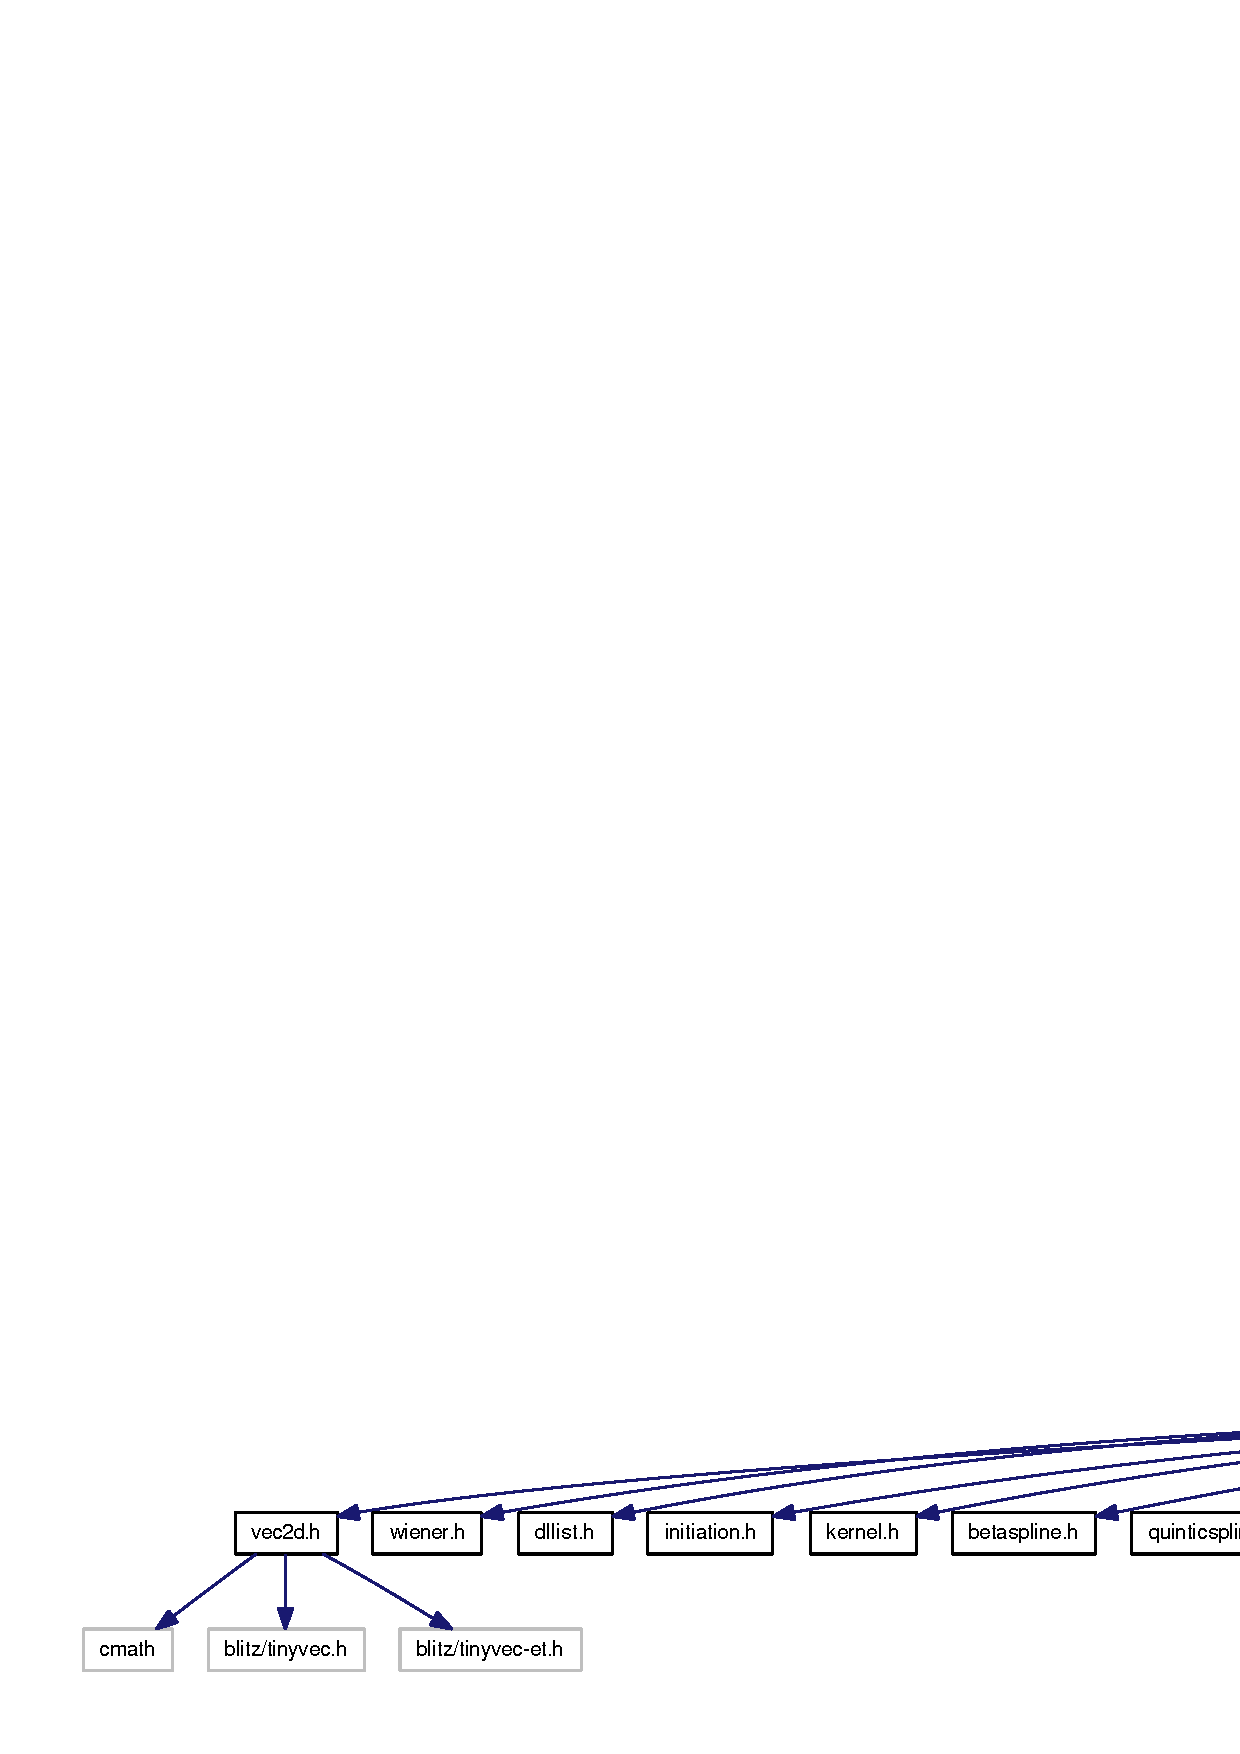
\includegraphics[width=420pt]{glbcls_8h__incl}
\end{center}
\end{figure}


This graph shows which files directly or indirectly include this file:\nopagebreak
\begin{figure}[H]
\begin{center}
\leavevmode
\includegraphics[width=420pt]{glbcls_8h__dep__incl}
\end{center}
\end{figure}


\label{_details}
\hypertarget{_details}{}
\subsection{Detailed Description}
Global class declarations. 

\begin{Desc}
\item[Author:]Xiangyu Hu $<$\href{mailto:Xiangyu.Hu@aer.mw.tum.de}{\tt Xiangyu.Hu@aer.mw.tum.de}$>$ 

changes by: Martin Bernreuther $<$\href{mailto:Martin.Bernreuther@ipvs.uni-stuttgart.de}{\tt Martin.Bernreuther@ipvs.uni-stuttgart.de}$>$ 

changes by: Andreas Mattes \end{Desc}
